%% ============================================================
%% ADY201m -- Phase 2 Project Planning Proposal
%% Springer Nature Journal LaTeX template (sn-jnl)
%% Group 11 -- Artificial Intelligence, FPT University HCM
%% ============================================================
\documentclass[pdflatex,sn-mathphys-num]{sn-jnl}

\usepackage{graphicx}%
\usepackage{amsmath,amssymb,amsfonts}%
\usepackage{xcolor}%
\usepackage{booktabs}%
\usepackage{array}%
\usepackage{tabularx}%
\graphicspath{{figures/}}

\raggedbottom

\begin{document}

\title[ADY201m Phase 2 Project Planning]{Project Planning Proposal:\\
Explainable CLV Ranking and Uplift-Aware Customer Targeting Across Retail Contexts}

\author*[1]{\fnm{Group~11}}\email{caophucai@gmail.com}

\affil*[1]{\orgdiv{Artificial Intelligence Program},
           \orgname{FPT University, Ho Chi Minh City Campus},
           \orgaddress{\city{Ho Chi Minh City}, \country{Vietnam}}}

\abstract{This proposal describes a ten-week Phase~2 Data Science project for ADY201m that
extends our Phase~1 Customer Lifetime Value (CLV) framework from a single online-retail dataset
to a multi-context study that connects \emph{value} with \emph{persuadability}. Phase~1 answered
\emph{who is valuable}; Phase~2 asks \emph{who is worth targeting}. We re-estimate an explainable
Hurdle--Semantic CLV model across UK online retail and US grocery contexts, then estimate
\emph{uplift} (incremental treatment effect) on a randomised supermarket SMS campaign, and finally
combine the two into a \emph{value-adjusted uplift} targeting rule. Following the mandated
PBL\,+\,RBL framework, the plan covers a full pipeline (ingestion, cleaning, EDA, feature
engineering, modelling, evaluation) in Python with supporting SQL analytics, more than five
predictive models compared against published baselines, an interactive targeting dashboard, and a
complete AI Audit Log demonstrating the \emph{Human Delta}. A central design commitment is
causal cleanliness: only the randomised X5 campaign is used for causal uplift, while coupon
redemption is explicitly excluded as a treatment.}

\keywords{Customer Lifetime Value, Uplift Modelling, RFM, Hurdle Model, Explainability,
Conformal Prediction, Cross-Context Generalisation, Campaign Targeting}

\maketitle

%% ============================================================
\section{Project Name and Requirements}\label{sec:req}
%% ============================================================
\textbf{Project name:} \emph{Explainable CLV Ranking and Uplift-Aware Customer Targeting Across
Retail Contexts -- From ``who is valuable'' to ``who is worth targeting''.}

\noindent\textbf{ADY201m requirements addressed:} a complete pipeline (Data $\rightarrow$ Cleaning
$\rightarrow$ EDA $\rightarrow$ Features $\rightarrow$ Modelling $\rightarrow$ Evaluation);
more than five predictive models compared against published baselines (eight CLV regressors plus
six uplift learners); SQL analytics integrated with Python; an interactive targeting dashboard
(Plotly Dash); a full AI Audit Log with Human Delta and at least three documented AI
hallucinations or oversimplifications; a 10--12 page Final Report typeset in the Springer Nature
single-column LaTeX template; and complete reproducibility (pinned environment and a single
\texttt{reproduce\_all} script).

%% ============================================================
\section{Business Understanding and Analytic Approach}\label{sec:biz}
%% ============================================================
Marketing budgets are finite, yet value-based targeting alone can be wasteful. A high-CLV customer
may purchase \emph{regardless} of any campaign (a ``sure buyer''), so retention dollars spent on
them yield little incremental return. Conversely, a mid-value customer who only re-purchases when
prompted is precisely the ``persuadable'' a campaign should reach. The business problem is
therefore to identify customers who are \emph{both valuable and incrementally responsive}, and to
do so in a way that transfers across retail contexts and remains explainable to marketers.

The analytic approach is structured as four progressively prescriptive layers:
\emph{Descriptive} (RFM, cohort activity, cross-context dataset profiling);
\emph{Diagnostic} (SQL segmentation; statistical tests on CLV between segments; treatment/control
balance audit); \emph{Predictive} (CLV regression and uplift estimation); and
\emph{Prescriptive} (a dashboard ranking customers by value-adjusted uplift for activation).

\noindent\textbf{The roles of CLV, Uplift, and Value-adjusted Uplift} are complementary, not
interchangeable: (i)~\textbf{CLV} is the predictive value lens, a regression label equal to future
revenue per customer; (ii)~\textbf{Uplift} is the causal lens, the incremental effect of a
randomised campaign; (iii)~\textbf{Value-adjusted uplift} ($\hat\tau_i\cdot\hat V_i$) is the
decision lens that fuses the two for budget-constrained activation. RQ1--RQ2 exercise CLV, RQ3
exercises uplift, and RQ4 exercises their fusion.

%% ============================================================
\section{Research Questions (RBL)}\label{sec:rq}
%% ============================================================
\begin{itemize}
\item \textbf{RQ1.} How robust is the explainable Hurdle--Semantic CLV framework when re-estimated
      across UK online retail and US grocery contexts? \emph{Method:} re-train the same pipeline on
      both datasets; compare Normalized Gini and Revenue Capture@10\% with bootstrap confidence
      intervals.
\item \textbf{RQ2.} Do semantic product profiles and behavioural sequence features add incremental
      value beyond RFM for CLV ranking, calibration, and interpretation? \emph{Method:}
      feature-group ablation with paired bootstrap tests; SHAP attribution per Hurdle stage;
      conformalized quantile regression coverage.
\item \textbf{RQ3.} On campaign data with treatment/control labels, does uplift-aware targeting
      outperform CLV-only, RFM-only, and response-model targeting? \emph{Method:} S/T/X-Learners and
      class transformation vs.\ response and random baselines; Qini AUC, AUUC, uplift@K.
\item \textbf{RQ4.} Can combining predicted value with uplift improve simulated campaign efficiency,
      and what transferable design principles follow for budget-constrained markets?
      \emph{Method:} value-adjusted uplift policy; profit / incremental-revenue simulation on the
      randomised test set with bootstrap CIs.
\end{itemize}

%% ============================================================
\section{Data Collection, Understanding, and Preparation}\label{sec:data}
%% ============================================================
\textbf{Three datasets with deliberately separated roles.}
(1)~\emph{Online Retail II} (UK e-commerce, Phase~1 baseline, read-only reuse): $\sim 0.8$M cleaned
transactions, $5{,}038$ observation customers.
(2)~\emph{Dunnhumby Complete Journey} (US grocery): $2{,}500$ households, $\sim 2.6$M transaction
lines over $102$ weeks; external CLV validation.
(3)~\emph{X5 RetailHero} (randomised SMS campaign): $200{,}039$ labelled clients with
\texttt{treatment\_flg}/\texttt{target} and $45.7$M pre-communication purchase lines; the sole
source of causal uplift.

\noindent\textbf{Causal-cleanliness commitment.} Dunnhumby coupon redemption is a post-campaign
outcome, not a clean treatment assignment; using it for causal uplift would invite selection bias.
We therefore restrict uplift to the randomised X5 design (audited treatment ratio $0.500$, raw
uplift $+3.3$ percentage points with a positive $95\%$ confidence interval) and use Dunnhumby only
for CLV validation.

\noindent\textbf{Preparation pipeline.} A shared normaliser maps each dataset to a common
transaction schema (customer, basket, date, product, quantity, revenue); observation and prediction
windows are split without leakage; the CLV label is future-window revenue
$Y_i=\sum_{t}\text{Revenue}_{i,t}$; and X5 features are aggregated from pre-communication purchases
only.

%% ============================================================
\section{Proposed Methodology and Tools}\label{sec:method}
%% ============================================================
The methodology has four modules. \textbf{Module~A (Hurdle CLV)} models value as
$\widehat{CLV}_i=p_i\cdot m_i$ with incidence $p_i=P(Y_i>0\mid X_i)$ and magnitude
$m_i=E[Y_i\mid Y_i>0,X_i]$ using gradient boosting and a lognormal correction.
\textbf{Module~B (Semantic profiling)} builds PPMI product co-occurrence embeddings via truncated
SVD and revenue-weighted customer taste vectors. \textbf{Module~C (Uplift)} estimates
$\tau_i=E[Y_i(1)-Y_i(0)\mid X_i]$ with S/T/X-Learners and class transformation. \textbf{Module~D
(Value-adjusted uplift)} scores customers by $\hat\tau_i\cdot\hat V_i$, where $\hat V_i$ is a
historical-spend value \emph{proxy}.

\noindent\textbf{Tools.} \texttt{pandas}, \texttt{numpy}, \texttt{scipy},
\texttt{scikit-learn}, \texttt{LightGBM}, \texttt{XGBoost}, \texttt{SHAP},
\texttt{scikit-uplift}, \texttt{matplotlib}; SQL via DuckDB; dashboard via Plotly Dash.
Headline metrics: Normalized Gini and Revenue Capture@10\% (CLV); Qini AUC and uplift@K (uplift);
profit@K (policy). Uncertainty via the percentile bootstrap and conformalized quantile regression.

%% ============================================================
\section{Data Analysis with SQL}\label{sec:sql}
%% ============================================================
Seven DuckDB queries support the four RQs across the datasets:
\begin{itemize}
\item \texttt{q1\_rfm\_per\_customer} --- R/F/M aggregation per customer/household (RQ1/RQ2);
\item \texttt{q2\_rfm\_segments} --- quintile RFM scores and named segments (RQ1);
\item \texttt{q3\_cohort\_activity} --- first-active-period $\times$ activity matrix (RQ1);
\item \texttt{q4\_zero\_rate\_by\_context} --- future-spend zero-rate and skew per context (RQ1);
\item \texttt{q5\_treatment\_balance} --- X5 treatment/control counts and target rates (RQ3);
\item \texttt{q6\_top\_value\_customers} --- top-decile value customers per context (RQ4);
\item \texttt{q7\_uplift\_decile\_overlap} --- overlap of top-response vs top-uplift deciles (RQ4).
\end{itemize}
\noindent\textbf{Deliverables:} one self-contained SQL notebook, seven CSV outputs, and a paragraph
linking each query to an RQ.

%% ============================================================
\section{Data Analysis with Python}\label{sec:py}
%% ============================================================
Eleven reproducible Python modules (\texttt{p2\_01}--\texttt{p2\_11}):
dataset audits; a shared feature pipeline (RFM, behavioural, sequence, and semantic-graph features);
cross-context comparison; CLV benchmark and ablation; SHAP and CQR; X5 uplift feature engineering;
uplift models; the value-adjusted policy comparison; bootstrap robustness; and an automatic
LaTeX-table generator that keeps the report numbers synchronised with the result files. Required
libraries are listed in a pinned \texttt{requirements.txt}.

%% ============================================================
\section{Data Visualisation}\label{sec:viz}
%% ============================================================
Core figures: cross-context dataset structure (zero-rate and tail, Fig.~\ref{fig:context});
revenue-capture and decile-calibration curves per context; stage-wise SHAP summaries; conformal
interval widths; X5 Qini curves; and targeting profit/incremental-revenue by budget. Each figure is
generated by a script and saved under \texttt{figures/} for direct inclusion in the report.

\begin{figure}[t]\centering
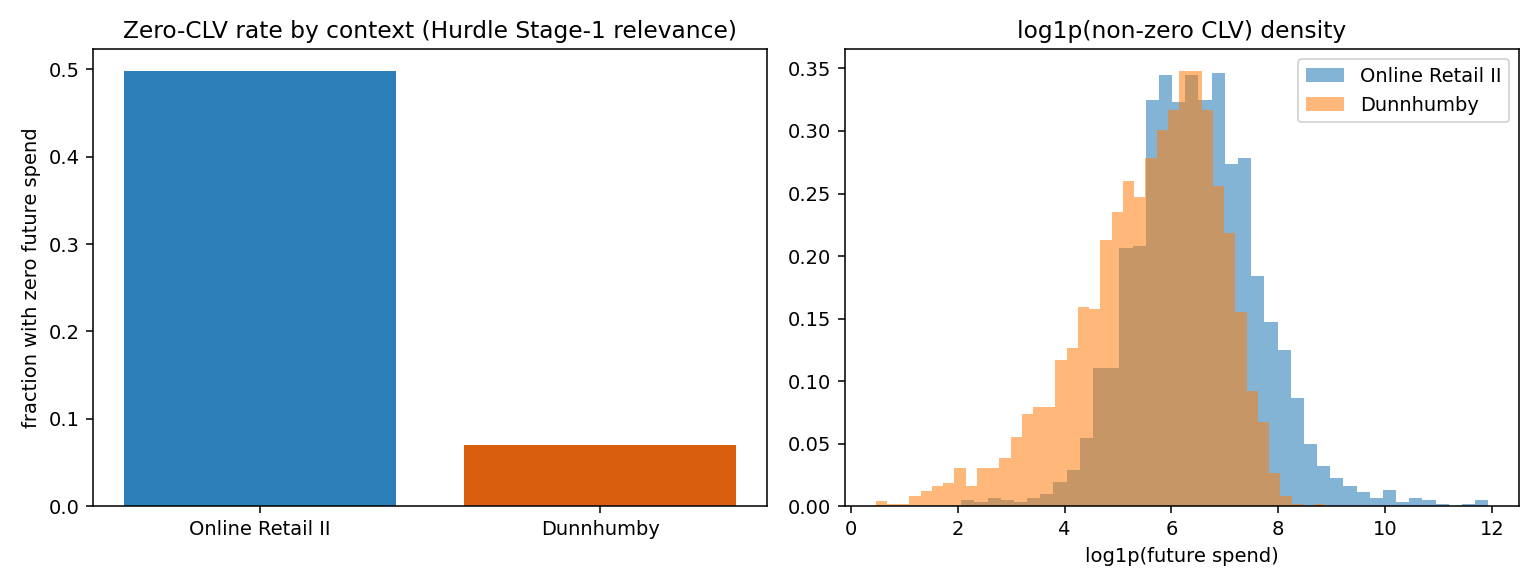
\includegraphics[width=\textwidth]{context_comparison.png}
\caption{Illustrative cross-context structure: e-commerce is zero-inflated and heavy-tailed,
grocery is near fully active and light-tailed -- motivating the RQ1 robustness test.}
\label{fig:context}
\end{figure}

%% ============================================================
\section{Predictive Modelling ($\geq$ Five Models)}\label{sec:models}
%% ============================================================
\textbf{CLV regressors (eight).} Mean and Monetary baselines, an RFM-score baseline, Ridge,
Random Forest, XGBoost, LightGBM, and the two-stage \emph{Hurdle} model (proposed). Metrics:
Normalized Gini, Revenue Capture@10/20\%, Precision@10\%, Spearman, MAE/RMSE, decile calibration.
\textbf{Uplift learners (six).} Random and Response baselines, S-Learner, T-Learner, class
transformation, and X-Learner. Metrics: Qini AUC, AUUC, uplift@10/20/30\%. Significance is assessed
by paired bootstrap differences (e.g.\ Hurdle vs.\ baseline; best uplift learner vs.\ response
model). This comfortably exceeds the five-model requirement and compares against published
baselines (BG/NBD-style monetary models for CLV; response and random models for uplift).

%% ============================================================
\section{Data Analysis with a Tool (Dashboard)}\label{sec:dash}
%% ============================================================
An interactive Plotly Dash application with four pages: (1)~cross-context CLV overview;
(2)~per-customer CLV ranking with conformal intervals; (3)~uplift Qini explorer; and
(4)~a value-adjusted targeting page that ranks the top-$K$ persuadable high-value customers under a
budget slider, with the simulated profit shown live. The dashboard consumes the CSV outputs of the
Python pipeline.

%% ============================================================
\section{Ten-Week Timeline and Deliverables}\label{sec:time}
%% ============================================================
\begin{itemize}
\item \textbf{W1} Dataset audits + feasibility gating (treatment balance, zero-rate, skew).
\item \textbf{W2} Shared feature engineering (RFM, behavioural, sequence, semantic).
\item \textbf{W3} CLV window design (week-level for grocery).
\item \textbf{W4} Cross-context CLV benchmark + ablation.
\item \textbf{W5} Explainability (SHAP per stage) + uncertainty (CQR).
\item \textbf{W6} X5 uplift feature engineering + baselines.
\item \textbf{W7} Advanced uplift learners (X-Learner, class transformation).
\item \textbf{W8} Value-adjusted uplift policy + profit simulation.
\item \textbf{W9} Robustness (bootstrap CIs) + transferable insights.
\item \textbf{W10} Report writing + reproducibility package.
\end{itemize}
\noindent\textbf{Deliverables:} cleaned data and shared feature tables; result CSVs and figures;
the AI Audit Log; a 10--12 page Springer report; a reproducibility bundle (\texttt{requirements.txt},
\texttt{reproduce\_all.sh}); and the dashboard.

%% ============================================================
\section{Risks, Mitigations, and AI Reflection}\label{sec:risk}
%% ============================================================
\textbf{Risk 1 -- causal misuse.} Treating coupon redemption as a campaign cause would bias uplift.
\emph{Mitigation:} restrict causal estimation to the randomised X5 design.
\textbf{Risk 2 -- data acquisition.} The X5 purchase history is large ($\sim 670$\,MB) and the link
unreliable. \emph{Mitigation:} a resumable, integrity-checked downloader; manual fallback.
\textbf{Risk 3 -- overclaiming.} Profit differences between policies may be within noise.
\emph{Mitigation:} bootstrap confidence intervals and explicit reporting of non-significant claims.
\textbf{Risk 4 -- leakage / isolation.} Phase~2 must not corrupt Phase~1 results.
\emph{Mitigation:} a separate project tree with a write-guard that refuses paths outside it.

\noindent\textbf{AI reflection (Human Delta).} AI assistance is used for ideation and drafting, but
every quantitative claim is recomputed from data, every cited reference is verified, and at least
three AI oversimplifications (e.g.\ ``response model is a strong targeting baseline'';
``coupon redemption is a valid treatment''; ``semantic features must improve ranking'') are
documented and corrected in the AI Audit Log with the reasoning behind each human decision.

\end{document}
